\chapter{Анализ литературы, патентов и обзор практики рецикла урана}\label{ch:ch1}

\section{Промышленный опыт}\label{sec:ch1/sec1}
Так как зарубежный опыт рецикла ядерного топлива исторически базируется на однократном использовании MOX-топлива, в данной работе будем опираться на Российский опыт возврата топлива в ЯТЦ \cite{international2003iaea}. К тому же, по части повторного использования урановой составляющей, отечественную ядерную индустрию можно считать глобальным лидером.  Эта практика вовлечения регенерата урана в топливные циклы энергетических реакторов базируется на смешении регенератов урана, извлекаемых из ОЯТ ВВЭР и ОЯТ транспортных реакторов с высоким содержанием $^{235}$U. Такая схема реализована для производства исходного сырья для изготовления топлива РБМК на заводе РТ-1 \cite{volkVozvratUranaIz2010}. Более того, этот вариант также апробирован для изготовления опытных ТВС для реакторов ВВЭР \cite{proselkovAnalizVozmozhnostiIspolzovaniya2003}, требующих более высокого уровня обогащения.

дообогащение регенерата до необходимого для повторного использования в энергетических ядерных реакторах уровня концентрации изотопа $^{235}$U может быть проведено на имеющихся в нашей стране промышленных разделительных мощностях, основанных на центробежном методе разделения. 

Согласно планам Росатома, в соответствии с глобальной стратегией ядерной индустрии, для обеспечения конкурентоспособности на рынке зарубежных топливных поставок для легководных энергетических реакторов, следует предложить решение, обеспечивающее замыкание (пускай пока что и частичное) ЯТЦ. Подразумевая несовместимость опции MOX-топлива с ВВЭР (отсутствует лицензия) и с многократным рециклом, а также выигрышность варианта REMIX категории В, который связан с необходимостью обогащения урана, сконцентрируемся на подборе каскадной схемы для производства НОУ, способной обеспечить наилучшее решение, отвечающее критериям и требованиям, которые будут сформулированы далее.

\subsection{Требования и их источники}\label{sec:ch1/sec1.1}

Наличие строгих ограничений требований обсуловлены нейтронно-физическими и радиационными свойствами четных изотопов из ряда $^{232,234,236}$U \cite{smirnovEvolutionIsotopicComposition2012, proselkovAnalizVozmozhnostiIspolzovaniya2003, dudnikovInfluence236UEfficacy2016}. Так, первый в этом ряду изотоп $^{232}$U является особенно опасным источником радиационного загрязнения из-за интенсивного гамма-излучения (2.6 МэВ), испускаемого дочерним короткоживущим $^{208}$Tl (3.65 мин.) \cite{matveevUran232EgoVliyanie1985,article}.
$^{232}$U вместе $^{234}$U превносят альфа-частицы в смесь гексафторида урана ($UF_6$ -- соединение, используемое в процессе обогащения урана \cite{orlovWayObtainUranium2015, orlovDesublimationPurificationTransporting2017}), вероятно, приводя к его диссоциации, что может привести к нежелательному появлению и дальнейшему осаждению в каскаде легких компоненты, такик как, например свободный фтор ($F_2$) \cite{kryuchkovObogashchennyyUranDobavleniem2007, bernhardtRadiationEffectsAlpha1958, shmelevRazrabotkaRaschetnoyModeli2012}. Однако вопрос о влиянии процессов образования новых компонент на закономерности массопереноса в разделительном каскаде до сих пор не достаточно изучен, если делать вывод о состоянии проблемы по открытым источникам.

$^{236}$U действует как паразитный поглотитель нейтронов, который препятствует цепной реакции. Этот эффект отравления реактора должен быть скомпенсирован в простейшем случае дополнительным количеством делящегося $^{235}$U в продукте. Записывая уравнение, для обеспечения требуемого эквивалента уровня обогащения по $^{235}$U, к заданной концентрации для случая обогащения природного урана необходимо обеспечить добавку, определяемую наличием $^{236}$U -- паразитного нейтронного поглотителя:
$C_{235 e q}^{P}=C_{235 n a t}^{P}+\delta C_{235}$, где $\delta C_{235}$ определяется функцией от содержания $^{236}$U в продукте:
$f\left(C_{236}^{P}\right)$, которая в простейшем случае соответствует $K_{236} \times C_{236}^{P}$. Здесь $K_{236}$ называется коэффициентом компенсации реактивности, значение которого может лежать в пределах 0.2--0.6 \cite{delagarzaMulticomponentIsotopeSeparation1961, delculAnalysisReuseUranium2009}. Стоит отметить, что изотоп $^{234}$U имеет тенденцию захватывать нейтрон и превращаться в делящийся $^{235}$U, что должно уменьшить необходимую компенсацию $^{236}$U \cite{dyachenkoIspolzovanieRegenerirovannogoUrana2012}, хотя это обычно не учитывается ввиду порядка малости. Содержание этих изотопов в низкообогащенном продукте может регулироваться различными стандартами, такими как, например, ASTM C996 - 15 \cite{c26committeeSpecificationUraniumHexafluoride}.

Итак, в обязательном порядке необходимо обеспечить:
\begin{enumerate}
  \item Соответствие необходимым требованиям (спецификациям), предъявляемые к свежему топливу в целом. Может быть сформулировано как удовлетворение ограничений на присутствие нежелательных четных изотопов урана (возникших при облучении топлива и последующем хранении). Так, в соответствии с распространенными стандартами для низкообогощенного урана:
  \begin{enumerate}
    \item концентрация изотопа $^{232}$U в конечном продукте строго ограничена $5\cdot10^{-7}$\%, а иногда и $2\cdot10^{-7}$\%.
    \item Отношение изотопов $^{234}$U и $^{235}$U в продукте не должно превышать 0.02.
    \item $^{236}$U должен быть скомпенсирован дополнительным количеством делящегося $^{235}$U в продукте. В простейшем случае это количество составляет $^{236}$U$\cdot0.29$.
  \end{enumerate}
  \item Вовлечение максимально возможной доли делящегося изотопа U-235 в топливный цикл, что соответствует критерию экономии природного урана
\end{enumerate}

Может быть дополнено следующими условиями (пожеланиями):
\begin{enumerate}
  \item Вывод из топливного цикла балластных вредных четных изотопов посредством изотопного разделения, в ходе которого и происходит "повторное" обогащение регенерата. Концентрации нежелательных искусственных изотопов могут быть минимизированы до некоторой степени, когда это возможно, для многократной переработки, избегая их накопления, применяя разбавление изотопными композициями без искусственных изотопов, а также схемы очистки (см. далее).
  \item Использовать восстановленный уран на единицу продукта НОУ в необходимой пропорции (~ 0.93), что соответствует возврату в топливный цикл в виде 1 кг свежего топлива 1 кг ОЯТ.
  \item Предотвращение нежелательных потерь работы разделения в ходе операции разделения изотопов.
  \item Избежание накопления высокотоксичных отходов.
  \item Предел допустимой концентрации $^{235}$U на любом из стадий производства может быть ограничен лицензией обогатительного комбината. Так, например на СХК, такое ограничение составляет 5\%, что запрещает б`ольшую часть схем, предназначенных для дообогащения регенерата.
\end{enumerate}

В целом, политика вовлечения регенерированного урана в ЯТЦ позволяет в базовом варианте достигать экономии природного урана на уровне 11--20\% и многократного снижения объемов высокоактивных радиоактивных отходов за счет переработки ОЯТ \cite{delculAnalysisReuseUranium2009}. Возможность же осуществлять многократный рецикл урана и курс на удлинение (пролонгацию) топливных кампаний, связанный с повышением исходного уровня обогащения, открывает перспективы еще б`ольших преимуществ повторного использования делящегося материала.
Все это делает актуальным разработки каскадных обогатительных схем, направленные на решение задачи вовлечения урановой составляющей отработанного топлива в топливный цикл легководных энергетических реакторов.


\section{Сравнительный анализ известных схем}\label{sec:ch1/sec2}

Ниже представлен анализ современных подходов к проблеме повторного обогащения регенерата, основанных на технологии газовой центрифуги (ГЦ) и достижениях каскадной теории разделения многокомпонентных смесей. Технология ГЦ на сегодня является лидирующей в промышленном производстве обогащенного урана.
Оставляя в стороне вопросы, связанные с химической переработкой для получения восстановленной урановой изотопной смеси, предлагается рассмотрение усовершенствованных конфигураций каскадов газовых центрифуг для повторного обогащения этой смеси. При этом, как и условились ранее, ограничимся регенерированным ураном, полученным из ОЯТ легководного энергетического реактора. В качестве примера будем рассматривать реактор российского дизайна -- ВВЭР.

\subsection{Основы теории разделения в каскадах}\label{sec:ch1/sec2.1}

\textcolor{red}{Базовые понятия (разделительный элемент, симметричн.-противоточное соединений, каскад) + основные уравнения (балансы, срез, коэффициенты разделения ступеней)}

Обогащение переработанного урана является задачей разделения изотопов многокомпонентной изотопной смеси, тогда как обогащение природного урана можно свести к более простой задачи разделения бинарной смеси. Сложность работы с многокомпонентным изотопным составом регенерата заключается в необходимости разработки теории исключительно для разделения многокомпонентных изотопных смесей (хотя это касается и разделения неурановых химических элементов, например вольфрама).

В области математического моделирования разделительных каскадов на сегодня разработан обширный набор расчетных моделей, которые могут быть применены к задаче по обогащению регенерата. В нашем случае для разделения смеси регенерата может быть применен ряд специальных теоретических моделей. Физико-математические модели каскадов основанны на фундаментальных законах, таких как закон сохранения вещества. Эти теоретические описания адекватны процессу разделения в реальных разделительных аппаратах, в качестве которых сегодня, как правило, используются газовые центрифуги. Однако модельные каскады позволяют заметно упростить изучение закономерностей изотопно-селективного массопереноса в разделительных каскадах.

Наиболее общая модель здесь называется «квазиидеальным» каскадом, где предполагается постоянство коэффициентов деления (срезов) потоков ($\theta$ делит входной поток на $\theta$ и $1 - \theta$ соответственно) по каскадным ступеням \cite{yamamotoMulticomponentIsotopeSeparating1978}. В настоящее время он используется в двух приближениях: со слабым обогащением (Q-каскад \cite{borisevichNewApproachOptimize2011, kolokoltsovDesignCascadesSeparating1970, zengQCascadeExplanation2012}) и неограниченным (произвольным) обогащением (квазиидеальный каскад \cite{sulaberidzeSpecialFeaturesEnrichment2006}). Обе математические модели предлагают выбор профиля потока в каскаде, следовательно, дают возможность добиться наиболее эффективного обогащения целевого компонента. Такой подход значительно упрощает как анализ закономерностей массообмена в каскаде для многокомпонентного разделения, так и соответствующий расчет. В исследованиях, как правило, когда обогащенный переработанный уран обогащается многопоточными схемами, часто используется модель R-каскада (Matched Abundance Ratio Cascade-MARC \cite{delagarzaMulticomponentIsotopeSeparation1961, woodEffectsSeparationProcesses2008, kazukihidaSimultaneousEvaluationEffects}). Это особый случай `квазиидеального' каскада. Здесь условие отсутствия смешивания выполняется для выбранной пары компонентов (например, это могут быть изотопы $^{235}$U и $^{238}$U). Еще раз подчеркнем, что все вышеупомянутые каскадные модели действуют как физически эквивалентные представления. 

Стоит упомянуть, что существует альтернативный подход к каскадному расчету, когда набор из шести уравнений включает 10 основных внутренних параметров:

$L_{i}, C_{i}, L_{i}^{\prime}, C_{i}^{\prime}, L_{i}^{\prime \prime}, C_{i}^{\prime \prime}, q_{i}, \theta_{i}, N_{i}, l_{i}$,

где $L_{i}, L_{i}^{\prime}, L_{i}^{\prime \prime}$ и $C_{i}, C_{i}^{\prime}, C_{i}^{\prime \prime}$ -- 
это потоки питания, продукта и отвала и их концентрации соответственно; $q_{i}$ -- коэффициент разделения; $\theta$ -- коэффициент деления потока на ступени (срез); $N_{i}$ -- число ступеней; и $l_{i}$ -- поток питания отдельной центрифуги.

Эти параметры связаны шестью уравнениями:
$\begin{array}{c}
  {L_{i}^{\prime}+L_{i}^{\prime \prime}=L_{i}} \\
  {L_{i}^{\prime} C_{i}^{\prime}+L_{i}^{\prime \prime} C_{i}^{\prime \prime}=L_{i} C_{i}} \\
  {q_{i}=\frac{(1-C_{i}^{\prime \prime}) C_{i}^{\prime}}{(1-C_{i}^{\prime}) C_{i}^{\prime \prime}}} \\
  {q_{i}=q_{i}\left(l_{i}, \theta_{i}\right)} \\
  {\theta_{i}=\frac{L_{i}^{\prime}}{L_{i}}} \\
  {l_{i}=\frac{L_{i}}{N_{i}}}
\end{array}$


Помимо этих 6$n$ соотношений, описывающих отдельные ступени, необходимо учитывать уравнение, связывающее межкаскадные потоки -- балансные уравнения, вид которых зависит от рассматриваемой схемы коммутации ступеней. Для каскада, показанного на рис. 1, эти уравнения записаны в виде:

$\begin{array}{c}
  {L_{1}=L_{2}^{\prime \prime}, \ldots ; L_{i}=L_{i-2}^{\prime}+L_{i+1}^{\prime \prime}, \ldots ;} \\
  {L_{1} C_{1}=L_{2}^{\prime \prime} C_{2}^{\prime \prime}, \ldots ; L_{i} C_{i}=L_{i-2}^{\prime} C_{i-2}^{\prime}+L_{i+1}^{\prime \prime} C_{i+1}^{\prime \prime}, \ldots}
\end{array}$

В дополнение к этим соотношениям необходимо учитывать граничные условия, относящиеся к внешним и внутренним параметрам. Например для симметричного противоточного каскада, они выражаются соотношениями: 
$P=L_{n}^{\prime} ; C_{P}=C_{n}^{\prime} ; W=L_{1}^{\prime \prime} ; C_{W}=C_{1}^{\prime \prime}$

, которые выполняются для каждой ступени каскада \cite{palkinDeterminationOptimalParameters2012}. Эти уравнения описывают отношения между соседними ступенями и, опираясь на ряд граничных условий, могут служить эффективной репрезентацией каскада.

\subsection{Основные модификации стандартного (ординарного) каскада, используемого для обогащения природного урана}\label{sec:ch1/sec2.2}
Далее представлен анализ современных подходов к проблеме повторного обогащения регенерата и соответствующий набор методов, основанных на технологии газовой центрифуги и достижениях теории каскадов. Эти методы соответствуют набору каскадных схем, предложенных для решения задачи возврата регенерированного урана в топливный цикл энергетических реакторов.

В работах \cite{sulaberidzeNekotoryhRazdelitelnyhProblemah2004,sulaberidzeProblemsRefinementRecycled4, smirnovKaskadnyeShemyZadachah2012} было показано, что отрицательное влияние указанных изотопов делает непригодным для обогащения регенерата ординарный каскад (каскад, имеющий три внешних потока – питание, отбор и отвал), используемый для обогащения природного урана.

Рассматривая же технические решения, позволяющие корректно (соблюдая все вышеозначенные условия) решить задачу обогащение регенерата. Начнем с ряда схем, основанных на базовом (ординарном/трехпоточном) каскаде.
Его можно применять, например, следующими способами (рис. \ref{fig:diagram1}) \cite{smirnovKaskadnyeShemyZadachah2012}:
\begin{enumerate}
  \item Совместное обогащение смесей природного и регенерированного урана.
  \item Производство обогащенной фракции из регенерата и последующее ее разбавление природной урановой смесью.
  \item Предварительное обогащение природного урана немного больше, чем необходимо для получения НОУ требуемого качества, с последующим разбавлением его регенератом.
\end{enumerate}

\begin{figure}[ht]
  \centerfloat{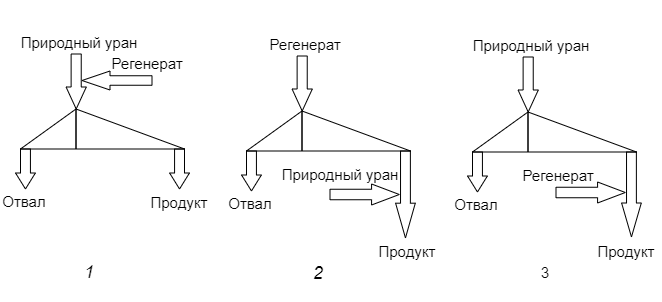
\includegraphics[scale=0.7]{cascades/diagram1}}
  \caption{Двойной каскад}\label{fig:diagram1}
\end{figure}

Соотношение между расходом регенерата и разбавителем природного происхождения определяется пределом содержания $^{232}$U в конечном продукте и компенсацией отрицательной реактивности $^{236}$U. В то же время концентрация $^{235}$U там не должна быть ниже, чем требуется для НОУ с определенными свойствами.

Основным преимуществом таких схем является простота реализации, поскольку нет необходимости в нестандартной модификации каскада. При этом, как недостаток можно выделить потери работы разделения, возникающие из-за смешения потоков с различными изотопными концентрациями $^{235}$U. 
Недостаточность такой простейшей модификации для решения задачи вовлечения регенерата в условия многократного рецикла будет показана в \ref{sec:ch1/sec3.1}.

Рассмотрим варианты практического применения таких схем. Схема 2 рисунка \ref{fig:diagram1} представляет собой возможный способ снижения накопления вредных изотопов в регенерате урана, как предложенно специалистами ОАО «Сибирский химический комбинат» (ОАО «СХК») в патенте № RU 2236053 \cite{SposobIzotopnogoVosstanovleniyaa}. Разбавление осуществляют следующим образом: сначала из регенерата в ординарном каскаде получают высокообогащенный уран (ВОУ), который затем разбавляют до нужного содержания изотопа $^{235}$U продуктом, не содержащим минорных изотопов. Например, это может быть природный уран или отвалы разделительного производства. Авторами патента показано, что оптимальная величина обогащения по изотопу $^{235}$U перед разбавлением составляет приблизительно 36\%. Следует подчеркнуть, что данную схему крайне затруднительно использовать практически. Наиболее критическими ее недостатками являются: 
\begin{enumerate}
  \item потери работы разделения при разбавлении ВОУ (количественные оценки величин затрат работы разделения для рассматриваемой схемы будут представлены в заключительном отчете по НИР).
  \item загрязненность разделительного оборудования примесными изотопами, в частности 232U, ухудшающим радиационную обстановку (смотри выше).
  \item необходимость обогащения материала до концентраций изотопа 235U, превышающих допустимые с точки зрения режима нераспространения величины.
\end{enumerate}

\subsection{Усовершенствованные конфигурации каскадов, например, с несколькими дополнительными внешними потоками (многопоточные схемы)}\label{sec:ch1/sec2.3}
Чтобы превратить базовый каскад в многопоточный, мы должны применить дополнительные питания или исходящие потоки побочных продуктов. Так, дополнительные входные потоки сырья действуют как разбавители, а при дополнительном удалении образуется очищенный промежуточный продукт.

\subsubsection{Применение дополнительных обособленных потоков питания}
Чтобы преодолеть недостатки, связанные с разделительными потерями упомянутых схем (рис. \ref{fig:diagram1}), трехпоточный каскад был модернизирован до многопоточного каскада с дополнительным потоком \cite{smirnovKaskadnyeShemyZadachah2012}. Здесь регенерат `направляется' (сублимируется с помощью конденсационно-испарительной установки из твердой в газообразную форму \cite{orlovDesublimationPurificationTransporting2017}) в каскад через отдельную точку подачи -- на ступень, отличную от ступени подпитки природной смесью (рис. !!!). Этот прием позволяет избежать неблагоприятных последствий смешения потоков с различными концентрациями $^{235}$U, располагая дополнительный входной поток там, где концентрации внешнего и внутреннего потоков в $^{235}$U совпадают (внешние потоки являются источником питания каскада; внутренние потоки -- потоки, циркулирующие внутри каскада). Поэтому очевидное практическое преимущество такого метода, по сравнению с предыдущими обычными схемами, связано с отсутствием потерь работы разделения \cite{smirnovKaskadnyeShemyZadachah2012, sulaberidzeQuasiidealCascadesAdditional2006}.

Использование большого количества природного урана для разбавления регенерата является обычным недостатком вышеупомянутых каскадных схем (рис. \ref{fig:diagram1} +!!!), поскольку необходимо, прежде всего, снизить содержание $^{232}$U в продукте. Тем не менее, при повторном использования топлива ВВЭР, такой подход может обеспечить значительную экономию природного урана $\approx$16\% только лишь на первом рецикле (а ведь это возможно осуществлять многократно, увеличивая экономию природного ресурса), как показано в оценках в \cite{smirnovEvolutionIsotopicComposition2012}. Но `полный' возврат ОЯТ в топливный цикл (использование 1 кг ОЯТ на 1 кг НОУ продукта) достижим в этом случае только для изотопных составов первого (иногда второго) рецикла, что означает невозможность с помощью такой схемы обеспечить требуемую пропорцию вовлечения регенерированного урана в условиях многократного рецикла \cite{smirnovApplyingEnrichmentCapacities2018}.
Для рассматриваемого каскада с двумя питаниями, начиная с третьего цикла, требуемый уровень использования регенерата становится невозможным из-за ухудшения изотопного состава урана и наличия ограничений на изотопы $^{232,236}$U.
Так, в \cite{smirnovApplyingEnrichmentCapacities2018} были рассчитаны экономия природного урана и работы разделения (РР) и показано, что для каждого цикла можно достичь примерно 20\% экономии природного урана до того, как к третьему циклу повторного использования происходит значительная деградация изотопного состава.
Чтобы повысить пределы экономии природного урана, оставаясь в рекомендованных пределах, мы должны искать альтернативный разбавитель. Например, это может быть обедненный уран (так называемые «хвосты» (или отвалы) -- побочный продукт процесса обогащения). Это может быть плодотворно использовано для частичной замены природного урана в качестве основного разбавителя, хотя этот материал часто рассматривается как «отходы». Такая конфигурация изображена на рис. !!!!. , описание же математической модели приведено в \cite{smirnovEnrichmentRegeneratedUranium2014}.
\textcolor{red}{Или можно как у Маслюкова запрудить мат.моделями?}
Основным преимуществом его использования является возможность б'ольшей экономии природного урана. В \cite{smirnovApplyingEnrichmentCapacities2018}, например, демонстрирется устойчивая экономию половины природного урана на каждом рецикле (ценой дополнительного расхода РР). При этом возможен выбор соотношения разбавителей и, как следствие, полученной экономии природного сырья и допущенного перерасхода РР. Эта особенность делает эту схему многообещающей, позволяя «настраивать» каскад для конкретных изотопных составов смесей и для текущих цен. Кроме того, такой вариант полезен для решения проблемы утилизации накопленных объемов обедненного урана \cite{smirnovEnrichmentRegeneratedUranium2014}. Поскольку гексафторид урана является довольно агрессивным веществом, его хранение связано с определенными затратами, и емкости для хранения следует время от времени заменять из-за коррозионных процессов \cite{fitchOPTIONSDISPOSALREAPPLICATION2009, oecdManagementDepletedUranium2001}.
Такая схема (рис. !!!!), как и предыдущая, могла бы обеспечить полный возврат урана в ядерный топливный цикл для двух начальных циклов, но это невозможно для серии последовательных циклов из-за быстрого накопления вредных четных изотопов и невозможности с помощью такой схемы очистить смеси от этих нежелательных компонентов \cite{smirnovApplyingEnrichmentCapacities2018}.

Таким образом, возникает проблема очистки изотопных составов.
Как мы можем заметить, во всех рассмотренных схемах заметное снижение содержания изотопов $^{232,234,236}$U в финальном НОУ достигается, прежде всего, за счет разбавления регенерата внутри каскада смесями, имеющими происхождение от природного урана (НОУ, ОГФУ, или сам природный уран). Далее будет показано, что приведенная классификация является условной, и будет предложена дихотомия, выделяющая схемы-разбавители и схемы-очистители (от четных изотопов). Итак, давайте опишем способы, как мы могли бы удалить нежелательные изотопы из системы, каким-то образом очистив смесь. Это может быть сделано со схемами, которые позволяют извлекать промежуточный продукт, или с составными схемами (несколько последовательных каскадов, например, двойной каскад). Остановимся на первых поподробнее.

\subsubsection{Применение дополнительных потоков отбора}
Схемы, называемые каскадами с промежуточным продуктом предназначены для «очистки» (по существу, все также при разбавлении природным ураном) от балластных изотопов представлена ниже (рис. !!) \cite{palkinAnaliticheskiyRaschetSoderzhaniya2007}. Здесь в качестве основного продукта получают НОУ требуемых характеристик, а в качестве промежуточного продукта получают композицию с пониженным содержанием нежелательных изотопов.
«Отфильтровывание» из смеси более высоких концентраций четных изотопов на первой стадии, позволяет получить больше преимуществ от увеличения количества делящегося $^{235}$U на второй -- при ее обогащении до товарного НОУ \cite{palkinSeparationUraniumIsotopes2010}.
Концентрация $^{235}$U в этом `очищенном' продукте составляет примерно 0,8-1,1 от его значения в исходном регенерате и регулируется как соотношением входящих потоков, так и положением промежуточной (дополнительноой) точки выходящего потока.
Как показано в \cite{palkinSeparationUraniumIsotopes2010}, в результате очистки содержание всех вредных изотопов значительно снижается. После чего, низкообогащенный уран с концентрациями $^{232,234,236}$U, удовлетворяющими требования ASTM для коммерческого продукта, может быть получен из очищенного промежуточного продукта путем его прямого обогащения. Рассматриваемая схема запатентована специалистами ОАО «СХК», патент № RU 2321544 \cite{shopenSposobPolucheniyaRazbavitelya2008}.
При этом важно заметить, что основной продукт НОУ каскада-очистителя также соответствует этим требованиям \cite{palkinSeparationUraniumIsotopes2010}. Следует отметить, что высокое качество очищенного регенерата достигается при малых потоках, в случае, когда необходимо выполнить требования к каждому из производимых НОУ.
Основным преимуществом здесь является то, что эта схема, обеспечивающая одновременное снижение $^{232,234,236}$U, практически не теряет РР и не требует загрязнения дополнительного каскада (будет обсуждаться далее в разделе составных схем).

Недостатки здесь заключаются в том, что эффект очистки обусловлен, прежде всего, уменьшением объема потока очищенного промежуточного продукта. Эффекта заметного снижения содержания минорных изотопов в дополнительном отборе можно добиться лишь при сильном разбавлении регенерата природным сырьем, в соотношениях, лежащих в диапазоне (1-25)/100 \cite{palkinSeparationUraniumIsotopes2010, smirnovKaskadnyeShemyZadachah2012}. Следовательно, данная схема не может обеспечить широкомасштабного возврата регенерированного урана в топливный цикл ВВЭР, ввиду малой удельной экономию природного урана.  Более того, такой подход демонстрирует снижение экономии природного урана. Кроме того, такой подход демонстрирует снижение экономии природного урана, и не позволяет вернуть весь ОЯТ (в соотношении к продукту 1:1).
В качестве материалов, которые необходимо очистить посредством такой схемы, можно рассматривать составы загрязненного урана природного состава, «хвостов» процесса обогащения и других, «загрязненных» урановыми $^{232,234,236}$U \cite{palkinSeparationUraniumIsotopes2010}. 
\textcolor{red}{Не пойму происхождение грязного ураном-234 природного урана. В районе реактора в Окло его добыли что ли? :)}

\subsection{Комбинации нескольких каскадов (составные схемы)}\label{sec:ch1/sec2.4}
Под составными схемами будем подразумевать коммутации единичных каскадов в единую составную структуру.

Приведенный критический анализ различных каскадных схем позволяет нам ближе рассмотреть возможные области применения и, таким образом, позволяет более осознанно выбирать конфигурацию для каждой обособленной практической задачи. То есть не представляется возможным остановиться на единственном универсально оптимальном варианте, а лишь можно отметить частные положительные стороны. Таким образом, этот обзор может быть использован в качестве основы для дальнейших научных, технических и технико-экономических обоснований крупномасштабного повторного использования ядерных материалов в различных топливных циклах. Такое исследование и будет проведено далее в данной диссертационной работе.

Рассмотрим принципы работы простейшего варианта составного каскада -- двойного каскада (рис. !!). Этот двойной каскад имеет более сложную модификацию, которая направлена на эффективное удаление $^{232}$U из каскада \cite{SosninYuChelcov, TehnicheskieResheniyaPo, SposobIzotopnogoVosstanovleniya}. В некоторых случаях она подразумевает использование газа-носителя (или буферного газа) \cite{prusakovCorrectingIsotopicComposition2008, SposobIzotopnogoVosstanovleniyab}. В первом каскаде (верхнем) $^{235}$U обогащается по легкой фракции, где также накапливается $^{232}$U. Затем, опционально, смесь объединяют с газом-носителем (буфером) и направляют во второй каскад, где она обогащается по $^{232,234}$U и концентрируется в загрязненной `отборной' части (вместе со вспомогательным буферным газом при наличии). В то же время НОУ желаемой обогащенной концентрации $^{235}$U направляется с тяжелой фракцией к другому выходу, в этой конфигурации представляющим из себя поток продукта.
Считается, что использование буферного газообразного соединения, которое является инертным (неактивным) к гексафториду урана -- рабочему газу в процессе центрифугирования, позволяет повысить эффективность отделения $^{232}$U из переработанного урана и уменьшить потери $^{235}$U. Идея применения этого газа с массовым числом, близким к $^{232}UF_6$, была выдвинута в \cite{SosninYuChelcov}, исходя из предположения, что такой газ мог бы служить матрицей-носителем для $^{232}UF_6$. В этом исследовании авторы предложили использовать фреон, поскольку среднее массовое количество этого соединения практически совпадает с массовым числом $^{232}UF_6$ (и ниже, чем в $^{235}UF_6$, что немаловажно).
Среди недостатков рассматриваемой схемы следует выделить следующие:
\begin{enumerate}
  \item оба каскада в схеме загрязнены изотопом 232U, что осложняет радиационную обстановку на разделительном производстве.
  \item в предлагаемой схеме принципиально отсутствует возможность снижения накопления изотопа 236U, негативное влияние которого на размножающие характеристики тепловыделяющих сборок (ТВС) требует дополнительного обогащения по изотопу 235U. При этом реализуемая эквивалентная концентрация 235U может быть заметно больше, чем в штатном топливе, что обуславливает дополнительные затраты работы разделения.
  \item для опции с газом-носителем, получаемый товарный продукт необходимо очищать от этого газа, что, очевидно, также приводит к увеличению удельных затрат.
\end{enumerate}

Таким образом, на практике мы считаем вариант без буферного газа предпочтительным, поскольку нет необходимости очищать смесь от буферного газа \cite{smirnovKaskadnyeShemyZadachah2012}. Среди недостатков таких схем следует отметить, что получение высокообогащенного урана с содержанием $^{235}$U более 20\%, что усложняет проблему соответствия международным стандартам обращения с делящимися материалами.
Такой подход помогает повторно обогащать переработанный уран, даже не разбавляя его сырьем, что делает его наилучшим вариантом с точки зрения экономии природного газа. Однако этот двойной каскад не может обеспечить решение проблемы `полного' (1:1) возврата. Она расходует значительно больше необходимого 0,93 кг регенерата на производство 1 кг свежего НОУ. Это означает, что для загрузки реактора, в котором используется переработанное топливо, необходимо будет использовать другой источник, скорее всего, таким ресурсом будет природный уран. Следовательно, в контексте закмыкания ЯТЦ по урановой составляющей и возврата в рассматриваемый реактор всего объема топлива, реальная экономия природного урана будет не 100\%, а в несколько раз меньше -- лучшем случае 15-20\%. И, как уже упоминалось, подобный принцип может быть реализован на практике без дополнительного агента -- газа-носителя.

В качестве необходимой модификации двойного каскада была предложена альтернативная каскадная схема, которая в принципе позволяет решить проблему полного возврата регенерата в цикл. В качестве такой альтернативы на рис.8 изображен случай, когда первая часть структуры увеличивает концентрацию 235U со всеми более легкими изотопами и направляет их (через выходящий поток в правой части на рисунке) ко второму каскаду, который будет концентрировать 232U и 234U в потоке загрязненного продукта [18]. Хотя на этот раз приготовленная композиция разбавляется НОУ для контроля концентраций 232,234U в допустимых пределах и для управления соотношением рециркулируемых материалов (для поддержания уровня полного возврата в ядерный топливный цикл).

Хотя этот вариант и кажется идеальным, цена хранения побочного продукта из загрязненной смеси слишком высока, что мгновенно делает схему нежизнеспособной, если нет способов избежать такого негативного побочного эффекта.
Однако в [49] автор предложил применить дополнительный каскад для производства НОУ из загрязненной смеси, сильно разбавленной обедненным ураном (которые имеют высокую концентрацию 235U ~ 20\%), чтобы получить конечный продукт в двух исходящих потоках и достичь значительной экономии природного урана (~ 38\%) даже для «грязной» композиции, которая уже была переработана пять раз. Расчеты показали, что такой подход позволяет производить НОУ коммерческого качества, расходуя определенное количество переработанного урана, в то же время отвечая стандартным спецификациям 232U (и условиям, установленным для других четных изотопов). В то же время, предлагаемая схема обеспечивает большую экономию природного урана, чем большинство схем обогащения переработанного урана. Это могло бы также обеспечить широкомасштабную «мобилизацию» обедненного урана.
Как мы видим, такие схемы также очень ценны как инструмент для возврата в ЯТЦ требуемого количества переработанного урана.

\section{Определение направлений дальнейших исследований}

\subsection{Поиск альтернативных конфигураций каскадов}
Дальнейшая работа предполагает подбор с помощью вычислительных экспериментов каскадов, которые могут быть использованы для операции повторного обогащения урана в рамках многократного рецикла. Кандидатами для такого поиска представляются схемы двух следующих типов.

\subsection{Исследование каскадов, использующих дополнительный отбор}
Схемы, производящие в дополнительном отборе очищенный от минорных четных изотопов полупродукт. Такая композиция с уменьшенным содержанием $^{232,234,236}$U, но со схожим с питающей смесью содержанием $^{235}$U, может быть направлена на вход схемы, подобной \ref{fig:Terminal_Dilution}, позволяя добиваться на выходе требуемого содержания по всем изотопам. Однако,  вариации таких схемы, обычно имеют дополнительные потоки питания, как представлено на рисунках \ref{fig:add}

\begin{figure}[ht]
  \begin{minipage}[b][][b]{0.49\linewidth}\centering
    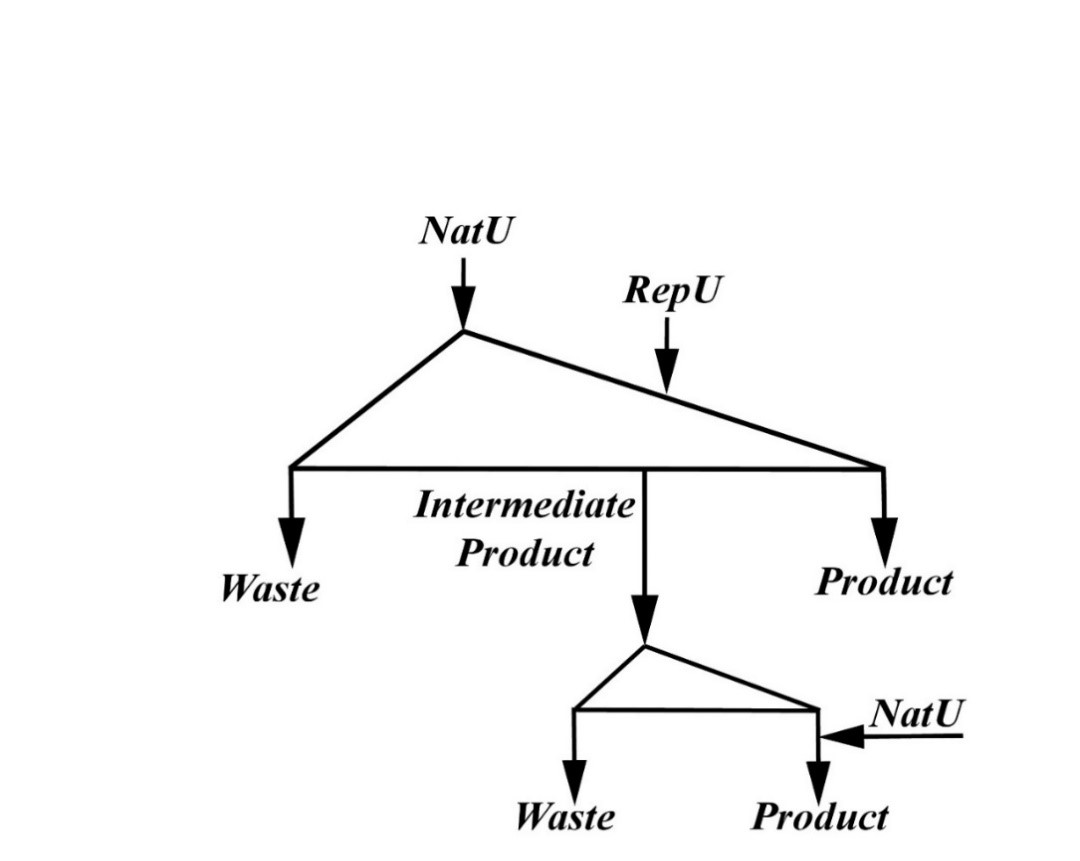
\includegraphics[width=0.9\linewidth]{cascades/add_p} \\ а)
  \end{minipage}
  \hfill
  \begin{minipage}[b][][b]{0.49\linewidth}\centering
    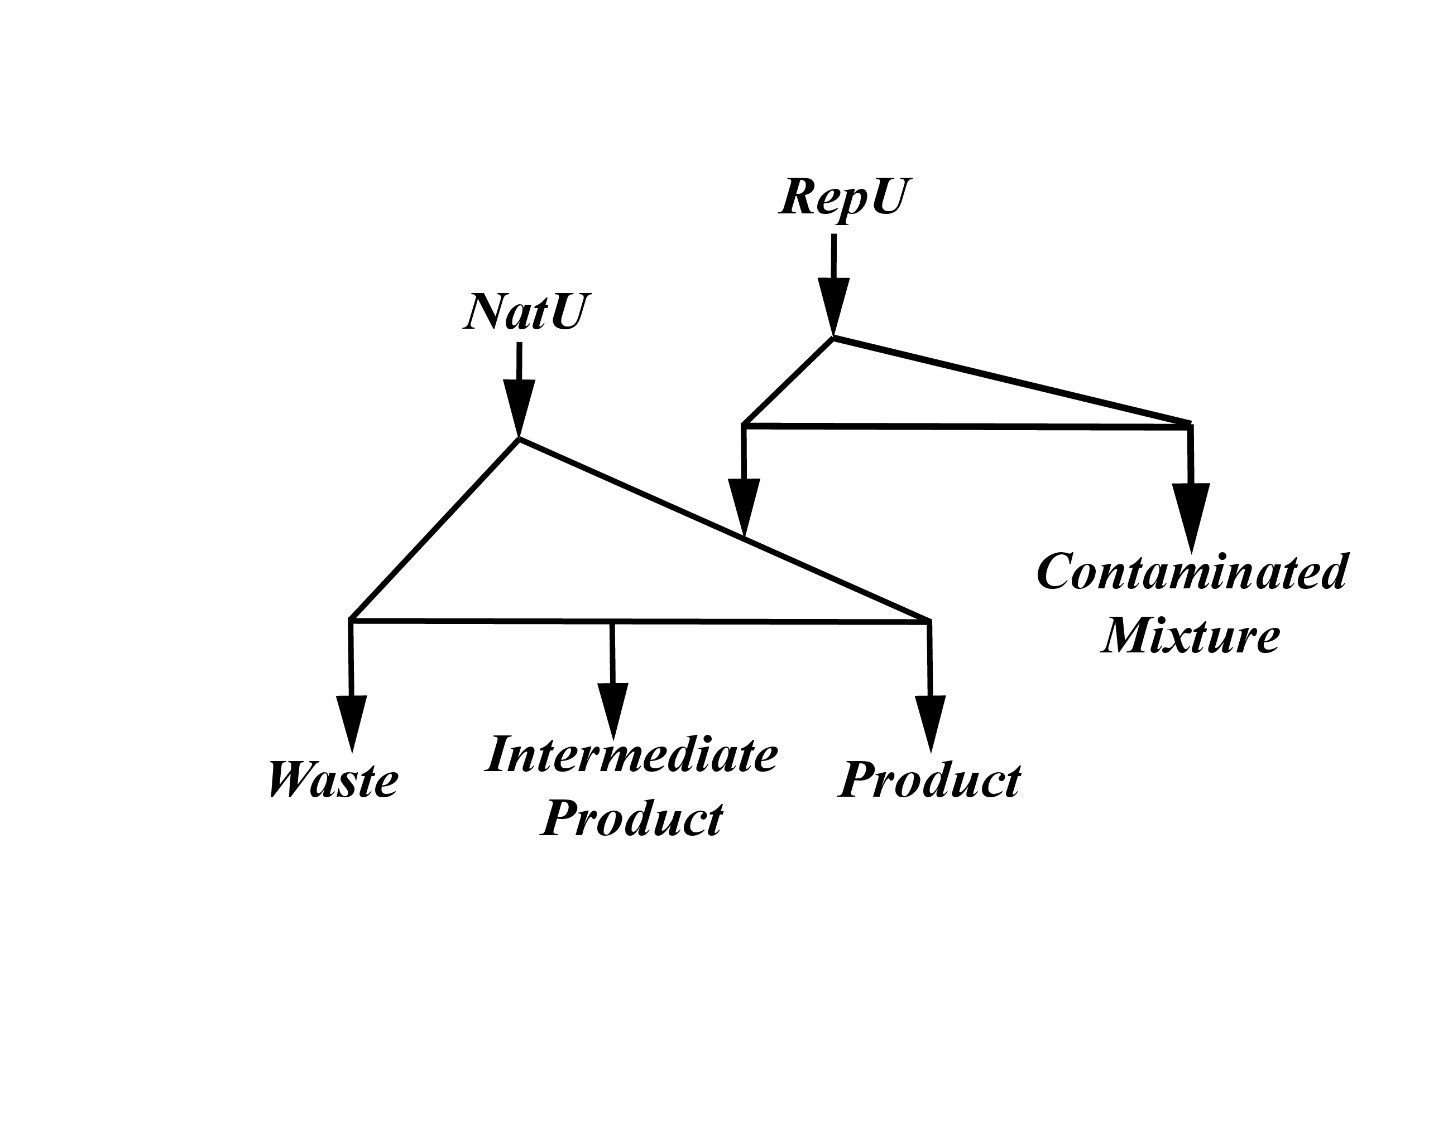
\includegraphics[width=0.9\linewidth]{cascades/add_p2} \\ б)
  \end{minipage}
  \caption{Каскады с дополнительным отбором}
  \label{fig:add}
\end{figure}


\subsection{Исследование каскадов, использующих смещение точки подачи питания}
С помощью модели квазиидеального каскада необходимо исследование конфигураций, использующих прием в виде варьирования точки подачи питания. Такие схемы тоже требуют анализа на пригодность к приложению в задачах дообогащения регенерированного урана до НОУ, которое может быть использовано в качестве топлива легководных реакторов. Как показано в \cite{palk_2013}, при смещении точки подачи питания каскада относительно оптимума, обеспечивающего минимально возможное число центрифуг, можно существенно изменить концентрацию нецелевых изотопов в отборе и отвале каскада. Такая особенность оптимизации может быть эффективно использована для очистки регенерированного урана от $^{232}$U.